\newpage
\phantomsection
{\bfseries ҒТАМР 84.13.21}
\hfill {\bfseries \href{https://doi.org/10.58805/kazutb.v.2.23-313}{https://doi.org/10.58805/kazutb.v.2.23-313}}

\sectionwithauthors{Г.К. Тайманова, Б.Б. Заутбек}{МҰНАЙ-ГАЗ КЕШЕНІ КӘСІПОРЫНДАРЫНДА САПА МЕНЕДЖМЕНТІ ЖҮЙЕСІН
ҚАЛЫПТАСТЫРУ ЖӘНЕ ДАМЫТУ}

\begin{center}
{\bfseries Г.К. Тайманова, Б.Б. Заутбек\envelope}

Әл-Фараби атындағы Қазақ ұлттық университеті, Алматы, Қазақстан,

\envelope Корреспондент-автор:
balzhan.zautbek02@gmail.com
\end{center}

Саланың қарқынды дамуы жағдайында сапаны тиімді басқару осы сектор
кәсіпорындарының табысты қызметінің маңызды элементіне айналады. Мақала
сапа менеджменті жүйесін қалыптастырудың негізгі аспектілерін анықтауға,
сондай-ақ, мұнай-газ саласының ерекшелігін ескере отырып, оны дамыту
әдістерін зерттеуге бағытталған.

Мақалада сапа менеджменті жүйесінің негізгі принциптері, ISO 9001:2015,
OHSAS 18001:2008, ISO 14001:2015 және ISO 45001:2018 және т.б.
стандарттары, сондай-ақ, мұнай-газ секторына тән нақты талаптар
қарастырылады. Мұнай-газ кешені кәсіпорындарында сапаны басқару
жүйелерін енгізудің табысты тәжірибелері талданады, сондай-ақ, осы
процесте компаниялардың алдында тұрған сын-қатерлер мен проблемалар
анықталады.

Мақалада мұнай-газ кешені кәсіпорындарында персоналды оқыту және сапа
мәдениетін дамыту мәселелері қарастырылады. Персоналды сапаны басқару
процестеріне тартудың және олардың рөлі жүйенің жалпы тиімділігіне қалай
әсер ететінін түсінуді қалыптастырудың маңыздылығына баса назар
аударылады.

Зерттеу барысында алынған тұжырымдар мұнай-газ кешені кәсіпорындарындағы
сапа менеджменті жүйесін одан әрі жетілдіруге құнды үлес болып табылады.
Энергетика секторындағы сапа менеджменті саласындағы болашақ зерттеулер
үшін негіз болады.

{\bfseries Түйін сөздер:} корпоративтік басқару, сапа менеджменті жүйелері,
SWOT-талдау, экологиялық көрсеткіштер, тиімділік, тұрақты жетілдіру.

\begin{center}
{\large\bfseries ФОРМИРОВАНИЕ И РАЗВИТИЕ СИСТЕМЫ МЕНЕДЖМЕНТА КАЧЕСТВА НА
ПРЕДПРИЯТИЯХ НЕФТЕГАЗОВОГО КОМПЛЕКСА}

{\bfseries Г.К. Тайманова, Б.Б. Заутбек\envelope}

Казахский национальный~университет~имени Аль-Фараби, Алматы, Казахстан,

e-mail: balzhan.zautbek02@gmail.com
\end{center}

В условиях динамичного развития отрасли, эффективное управление
качеством становится критически важным элементом успешной деятельности
предприятий данного сектора. Статья направлена на выявление ключевых
аспектов формирования системы менеджмента качества, а также на
исследование методов её развития с учетом специфики нефтегазовой
отрасли.

В статье рассматриваются основные принципы системы менеджмента качества,
стандарты ISO~9001:2015, ISO~14001:2015 и~ISO~45001:2018 и др., а также
специфические требования, характерные для нефтегазового сектора.
Анализируются успешные практики внедрения систем управления качеством на
предприятиях нефтегазового комплекса, а также выявляются вызовы и
проблемы, с которыми сталкиваются компании в этом процессе.

В статье также рассматриваются вопросы обучения персонала и развития
культуры качества на предприятиях нефтегазового комплекса. Акцент
делается на важности вовлечения персонала в процессы управления
качеством и формирования понимания того, как их роль влияет на общую
результативность системы.

Полученные в ходе исследования выводы представляют собой ценный вклад в
дальнейшее совершенствование систем менеджмента качества на предприятиях
нефтегазового комплекса, а также служат основой для будущих исследований
в области управления качеством в энергетическом секторе.

{\bfseries Ключевые слова:} корпоративное управление, системы менеджмента
качества, SWOT-анализ, экологические показатели, эффективность,
постоянное совершенствование.

\begin{center}
{\large\bfseries FORMATION AND DEVELOPMENT OF A QUALITY MANAGEMENT SYSTEM AT THE
ENTERPRISES OF THE OIL AND GAS COMPLEX}

{\bfseries G.K. Taimanova, B.B. Zautbek\envelope}

Al-Farabi Kazakh national university, Almaty, Kazakhstan,

e-mail: balzhan.zautbek02@gmail.com
\end{center}

In the context of the dynamic development of the industry, effective
quality management is becoming a critical element of the successful
operation of enterprises in this sector. The article aims to identify
the key aspects of the formation of a quality management system, as well
as to study the methods of its development, taking into account the
specifics of the oil and gas industry.

The article discusses the basic principles of the quality management
system, ISO 9001:2015, ISO 14001:2015 and ISO 45001:2018 standards,
etc., as well as specific requirements specific to the oil and gas
sector. The successful practices of implementing quality management
systems at oil and gas enterprises are analyzed, as well as the
challenges and problems faced by companies in this process are
identified.

The article also discusses the issues of personnel training and the
development of a quality culture at oil and gas enterprises. The
emphasis is on the importance of involving personnel in quality
management processes and developing an understanding of how their role
affects the overall effectiveness of the system.

The findings obtained in the course of the study represent a valuable
contribution to the further improvement of quality management systems at
oil and gas enterprises, and also serve as a basis for future research
in the field of quality management in the energy sector.

{\bfseries Keywords:} corporate governance, quality management systems,
SWOT analysis, environmental performance, efficiency, continuous
improvement.

\begin{multicols}{2}
{\bfseries Кіріспе.} ҚР бюджеті мен төлем балансының басым бөлігін
қалыптастыра отырып, мұнай-газ өндіру саласы мемлекет ауқымында түйінді
және стратегиялық маңызды болып табылады. ҚР-дағы мұнай-газ саласы ел
аумағында және одан тыс жерлерде мұнай мен газды өндіруді, өңдеуді,
жеткізуді және өңдеуді қамтиды. Мұнай-газ өндіру кешені республика
бюджетін қалыптастыру үшін стратегиялық маңызды компонент болып
табылады, бұл сала кәсіпорындарындағы бизнес-процестерді жетілдіру және
оңтайландыру тұрғысынан көптеген зерттеулерге негізделген. Атап
айтқанда, СМЖ енгізуді американдық мұнай институтының (API) Specq1
талаптары негізінде жүзеге асырған жөн, өйткені мұндай жүйе бірден үш
стандарттың өлшемдерін қанағаттандырады: APISpecQ1, ISO/TS 29001:2010,
ISO 9001: 2008. Осылайша, кәсіпорын өзінің бәсекелестік қуатын арттырып
қана қоймай, кейіннен пайданы ұлғайта алады. Негізгі тұтынушылар
тарапынан қолдауды қалыптастырады {[}1{]}. Американдық мұнай
институтының сапа менеджменті жүйесінің API Specification Q2 талаптарына
сәйкес мұнай сервисі активтерін сертификаттау мұнай сервисі активтері
қызметтерінің сапасын API мұнай-газ саласындағы халықаралық
стандарттардың озық және дамыған практикасына сәйкестік деңгейіне дейін
арттыру мақсатында басталды. Мұнайдың дәлелденген қоры бойынша Қазақстан
әлемде 12-орында - 3.9 млрд тонна. Табиғи газ қоры 2.7 трлн текше метрді
құрайды -- әлемдегі 14 орын. Қазақстанның дәлелденген мұнай және
конденсат қорларын өндірудің ағымдағы деңгейінде 45 жылдан астам уақытқа
жеткілікті (1-кесте) {[}2{]}.
\end{multicols}

\begin{table}[H]
\caption*{1-кесте - Елдер бойынша дәлелденген мұнай және конденсат қорлары, млрд. тонна}
\centering
\begin{tabular}{|l|p{0.18\textwidth}|p{0.2\textwidth}|l|}
\hline
\textbf{Мемлекеттер} & \textbf{Дәлелденген мұнай қорлары, млрд. тонн.} & \textbf{Жетістік деңгейі неше жыл, жыл} & \textbf{Әлемдік қордан, \%} \\ \hline
Венесуэла & 48 & 500 & 17,5 \\ \hline
Сауд Арабиясы & 40,9 & 73,6 & 17,2 \\ \hline
Канада & 27,1 & 89,4 & 9,7 \\ \hline
Иран & 21,7 & 139,8 & 9,1 \\ \hline
Ирак & 19,6 & 96,3 & 8,4 \\ \hline
Ресей & 14,8 & 27,6 & 6,2 \\ \hline
Кувейт & 14 & 103,2 & 5,9 \\ \hline
Біріккен Араб Әмірліктері & 13 & 73,1 & 5,6 \\ \hline
АҚШ & 8,2 & 11,4 & 4 \\ \hline
Ливия & 6,3 & 339,2 & 2,8 \\ \hline
Нигерия & 5 & 56,1 & 2,1 \\ \hline
\textbf{Қазақстан} & \textbf{3,9} & \textbf{45,3} & \textbf{1,7} \\ \hline
Қытай & 3,5 & 18,2 & 1,5 \\ \hline
Катар & 2,6 & 38,1 & 1,5 \\ \hline
Бразилиа & 1,7 & 10,8 & 0,7 \\ \hline
Алжир & 1,5 & 25 & 0,7 \\ \hline
Ангола & 1,1 & 16,1 & 0,4 \\ \hline
Норвегия & 1 & 10,8 & 0,5 \\ \hline
Әзірбайжан & 1 & 26,7 & 0,4 \\ \hline
Мексика & 0,9 & 8,7 & 0,4 \\ \hline
\end{tabular}
\end{table}

\begin{table}[H]
\caption*{2-кесте - 2021-2022 жылдар кезеңінде ҚР-дағы мұнай және газ өндіру бойынша ірі компаниялардың рейтингі}
\centering
\begin{tabular}{|p{0.2\textwidth}|p{0.2\textwidth}|p{0.2\textwidth}|p{0.2\textwidth}|}
\hline
Компания & 2021 жылы іске асыру көлемі, млн тг. & 2020 жылы іске асыру көлемі, млн тг. & Өсу қарқыны, \% \\ \hline
"ҚазМұнайГаз" ҰК & 5838793 & 3624964 & 61 \\ \hline
Қарашығанақ Петролиум Оперейтинг Б. В. & 1461823 & 1073920 & 36 \\ \hline
North Caspian Operating Company N.V. & 3737330 & 1871516 & 100 \\ \hline
Nostrum (ТОО «Жаикмунай») & 83197 & 72654 & 15 \\ \hline
«Матен Петролеум» & 157686 & 92339 & 71 \\ \hline
\end{tabular}
\end{table}

\begin{multicols}{2}
Нарықта бәсекеге қабілеттілікті арттыру үшін компаниялар
бизнес-процестерді тиімді басқаруды жүзеге асыруы және сапа менеджменті
жүйесін (СМЖ) енгізуі қажет. Егер сапа менеджменті жүйесі қабылданған
халықаралық стандарттарға сәйкес келсе, кәсіпорынның қызметі тиімді деп
саналуы мүмкін. Сапа жүйесінің стандарттары мен сәйкестік критерийлерін
таңдау кәсіпорынның түпкі мақсатына байланысты және мүдделі тұлғалардың
пікірін ескере отырып жүзеге асырылады. Сапаны басқаруды стандарттаудан
бөлек қарастыруға болмайды, оның нормативтік базасы компанияларға сапаны
бағалауға, тексеру процедурасы мен критерийлерін белгілеуге мүмкіндік
береді {[}3{]}.

{\bfseries Материалдар мен әдістер.} Мұнай-газ компанияларында енгізілген
сапа менеджменті жүйелері бизнес-процестерді, өнім сапасын жетілдіруді
қамтамасыз етеді және кәсіпорындар қызметінің түпкілікті нәтижелеріне өз
әсерін тигізеді. Бұл зерттеудің өзектілігін негіздейді.

Мұнай-газ секторы тәуелсіз компаниялардың кешені болып табылады, олардың
қызметі құрылатын тауардың бүкіл өмірлік циклін қамтиды. Өмірлік циклдің
барлық кезеңдерін сапа менеджменті жүйесінің көмегімен бағалау және
бақылау қажет, арнайы рәсімге және алдын ала белгіленген бағалау
критерийлеріне сәйкес халықаралық сапа стандарттарын енгізу қажет.
RAEX-Europe тәуелсіз Еуропалық рейтингтік агенттігінің деректері бойынша
мұнай-газ өндіру саласындағы өнімді өткізу көлемі бойынша Қазақстанның
ірі компанияларының рейтингі жасалды (2-кесте) {[}4{]}.

«ҚазМұнайГаз» ҰК АҚ компаниясы ҚР-дағы мұнай-газ өндіру саласындағы
компаниялар тізімінің көшбасшысы болды. Мұнай-газ компаниясы қандай
стандарттарды қолданатынын қарастырайық. Кәсіпорындар құжаттаманы және
сапа стандарттарының көпшілігін дербес әзірлейді. 2006 жылдан бастап
ҚМГ-да ISO 9001:2015, OHSAS 18001:2018, ISO 14001:2015 және ISO
45001:2018 талаптарына сәйкес сапа, қоршаған ортаны қорғау, денсаулықты
қорғау және еңбек қауіпсіздігін қамтамасыз ету саласында басқарудың
интеграцияланған жүйесі енгізілді {[}5{]}. Энергия тұтынудың едәуір
деңгейі бар компания ISO 50001:2018 стандартына сәйкес сертификатталған.
Біріктірілген басқару жүйесінің тиімділігін тәуелсіз аудиторлар үнемі
растайды. Олар компания ішінде де, ол жұмыс істейтін кәсіпорындарда да
таралады {[}6{]}.

ҚМГ корпоративтік басқару жүйесі кәсіпорындардың қызметін басқару мен
бақылауды, сондай-ақ, акционерлер, Директорлар кеңесі, басқарма және
мүдделі тараптар арасындағы өзара қарым-қатынас жүйесін қамтамасыз
ететін процестердің жиынтығы болып табылады. 2015 жылдан бастап қазіргі
уақытқа дейін ҚМГ «Самұрық-Қазына» АҚ Басқармасының шешімімен бекітілген
ҚМГ корпоративтік басқару Кодексін енгізу бойынша жұмыс жүргізуде (2015
жылғы 27 мамырдағы №22/15 хаттама). ҚМГ корпоративтік басқару кодексінің
мақсаты корпоративтік басқаруды жетілдіру, басқарудың ашықтығын
қамтамасыз ету, ҚМГ-ның тиісті корпоративтік басқару стандарттарын
ұстануға бейілділігін растау болып табылады. Осылайша, ҚМГ-да
корпоративтік басқару құрылымы құрылады (1-сурет).
\end{multicols}

\begin{figure}[H]
	\centering
	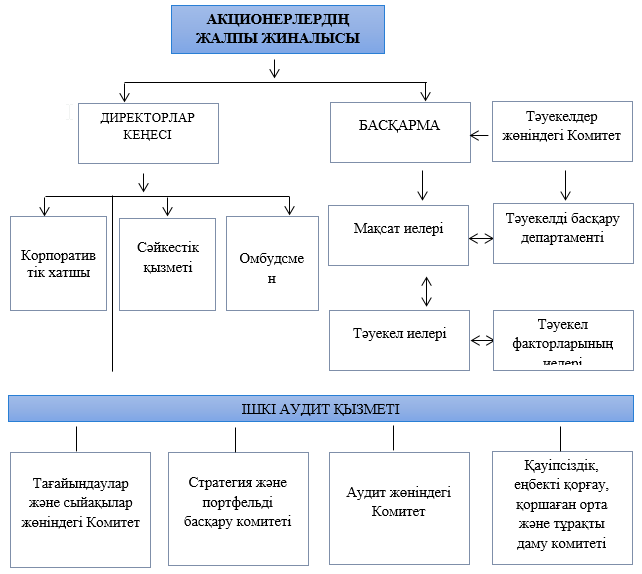
\includegraphics[width=0.7\textwidth]{assets/1361}
	\caption*{1-сурет - ҚМГ-дағы корпоративтік басқару құрылымы}
\end{figure}

\begin{multicols}{2}
Тұтастай алғанда, компаниядағы корпоративтік басқаруды жетілдіру
үздіксіз циклдік процесс болып табылады, оның негізгі кезеңі тәуелсіз
тараптан рейтинг және жақсарту бойынша тиісті ұсыныстар алу болып
табылатындығының айқын көрінісін келесі 2-суреттен көре аламыз {[}7{]}.
\end{multicols}

\begin{figure}[H]
	\centering
	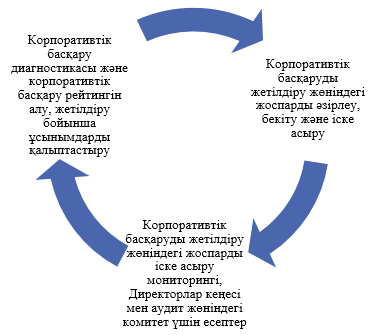
\includegraphics[width=0.5\textwidth]{assets/1362}
	\caption*{2-сурет - Корпоративтік басқару жүйесін дамыту}
\end{figure}

\begin{multicols}{2}
2020-2022 жылдар кезеңінде «ҚазМұнайГаз» ҰК АҚ жұмыс тиімділігінің
көрсеткіштерінің өзгеру динамикасын қарастырайық (3-кесте). Кез келген
мұнай саласындағы компанияның көрсеткіштерінің өзгеру динамикасы мұнай
бағасына, сонымен қатар, мұнай өндіру, тасымалдау, т.б. процестерге
әсерін тигізеді {[}8{]}.
\end{multicols}

\begin{table}[H]
\caption*{3-кесте -- «ҚазМұнайГаз» ҰК АҚ-ның 2020-2022 жылдардағы тиімділік көрсеткіштері}
\centering
\begin{tabular}{|p{0.5\textwidth}|l|l|l|}
\hline
Тиімділік көрсеткіші & 2020 & 2021 & 2022 \\ \hline
Тұтынушылардың өндіруге, тасымалдауға және өңдеуге орташа қанағаттануы, ұпайлар & 4,5 & 4,6 & 4,8 \\ \hline
Материалдық емес активтер, млн. тг. & 168,481 & 889,491 & 918,253 \\ \hline
Күрделі салымдар, млн. тг. & 432806,29 & 480677,1 & 441861,86 \\ \hline
\end{tabular}
\end{table}

\begin{multicols}{2}
{\bfseries Нәтижелер мен талқылау.} Мұнай-газ кешені кәсіпорындары
тұтынушыларының мұнай мен газды өндіруге, тасымалдауға және өңдеуге
орташа қанағаттануы бес балдық шкала бойынша қаралды және екі жыл ішінде
0,3 пунктке өсті. Клиенттердің қанағаттануы сапамен тығыз байланысты
болғандықтан, компаниядағы өнімдер мен қызметтердің сапасын жақсартуға
болады деген қорытынды жасауға болады.

Компанияның материалдық емес активтері жыл сайын өсіп келеді. 2022 жылы
2021-мен салыстырғанда материалдық емес активтердің құны 3,23\%-ға
немесе 28,762 млн теңгеге өсті. Бұл кәсіпорындардың жыл сайынғы
есептілігіне сәйкес сауда маркасының құнының өсуіне байланысты болуы
мүмкін. Ұйымның күрделі салымдары жалпы төмендеу үрдісіне ие. 2 жыл
ішінде ұйым шығындарды 8,1\%-ға оңтайландырды {[}9{]}.

ҚМГ республиканың ірі өнеркәсіптік кәсіпорындарының бірі бола отырып,
Қауіпсіз еңбек жағдайларын қамтамасыз етуге және компанияның өндірістік
объектілері қызметінің аудандарында тұратын персонал мен халықтың
денсаулығын қорғауға көп көңіл бөледі. Осыған сәйкес ұйым еңбек қызметі
үшін қауіпсіз жағдайлар жасауы керек және жұмыс орнында еңбекті қорғауды
қамтамасыз ету үшін ең жоғары стандарттарды енгізуі керек. Әрі қарай,
2020-2022 жылдар кезеңіндегі еңбекті қорғау мен өнеркәсіптік
қауіпсіздіктің негізгі көрсеткіштерін қарастырыңыз (4-кесте).
\end{multicols}

\begin{table}[H]
\caption*{4-кесте -- «ҚазМұнайГаз» ҰК АҚ-ның 2020-2022 жылдардағы тиімділік көрсеткіштері}
\centering
\begin{tabular}{|p{0.5\textwidth}|l|l|l|l|l|}
\hline
ЕҚ және ӨҚ негізгі көрсеткіштері & Өлшем бірлігі & 2020 & 2021 & 2022 & \% \\ \hline
Жазатайым оқиғалар & Оқиға & 30 & 28 & 35 & 25 \\ \hline
Жазатайым оқиғалар кезінде зардап шеккендер & Адам & 32 & 32 & 36 & 12,5 \\ \hline
Соның ішінде өлім & Адам & 0 & 3 & 1 & -67 \\ \hline
Жол-көлік оқиғалары & Оқиға & 14 & 22 & 24 & 9 \\ \hline
\end{tabular}
\end{table}

\begin{multicols}{2}
Денсаулық сақтау, өнеркәсіптік қауіпсіздік және қоршаған ортаны қорғау
жөніндегі менеджмент жүйесі Қазақстан Республикасы заңнамасының, ISO
14001:2015 және ISO 45001:2018 салалық және халықаралық стандарттарының
талаптарына сәйкес, үздік әлемдік тәжірибелер мен тәсілдерді,
Халықаралық Мұнай және газ өндірушілер қауымдастығының (International
Association of Oil \& Gas Producers, IOGP) ұсынымдарын пайдалана отырып
әзірленді), көшбасшылық, мақсатқа жету, тәуекелдерді басқару және
үздіксіз жетілдіру сияқты іргелі принциптерге негізделген 10 негізгі
элементті қамтиды.

Басқару жөніндегі мақсаттар ҚМГ компаниялар тобының даму стратегиясымен
тікелей байланысты. ҚМГ-ның 2031 жылға дейінгі Даму стратегиясы
экологиялық жауапкершілікті арттыру жөніндегі стратегиялық бастамаларды
көздейді. Қоршаған ортаны қорғау бөлігінде ҚМГ компаниялар тобы үшін
басым бағыттарға атмосфералық ауаға шығарындыларды басқару және газдың
алауды жағуын қысқарту, су ресурстарын, Өндіріс қалдықтарын басқару және
жерді рекультивациялау жатады {[}10{]}.

ҚМГ осы салада экологиялық көрсеткіштерді жақсарту және ашықтық пен
ашықтықты қамтамасыз ету бойынша жүргізіліп жатқан жұмыстардың
нәтижесінде дүниежүзілік жабайы табиғат қорының (WWF), CREON Group және
талдамалық кредиттік рейтингтік агенттіктің тәуелсіз сарапшыларын
бағалау нәтижелері бойынша Қазақстан Республикасы Мұнай-газ
компанияларының экологиялық ақпаратының ашықтығы рейтингінде алтыншы жыл
қатарынан бірінші орын алады. Экологиялық көрсеткіштердің жақсаруы
5-кестеде көрсетілген {[}11{]}.
\end{multicols}

\begin{table}[H]
\caption*{5-кесте - Экологиялық көрсеткіштер, б.з. 1 мың тоннаға тонна}
\centering
\begin{tabular}{|l|l|l|l|}
\hline
Жыл & 2020 & 2021 & 2022 \\ \hline
Шығарындылардың қарқындылығы, SO2 & 0,23 & 0,22 & 0,21 \\ \hline
Шығарындылардың қарқындылығы, NO2 & 0,22 & 0,24 & 0,31 \\ \hline
Шикі газды жағу қарқындылығы & 2,2 & 2,1 & 1,5 \\ \hline
Шикі газды кәдеге жарату деңгейі, \% & 98 & 98 & 98,8 \\ \hline
\end{tabular}
\end{table}

\begin{multicols}{2}
Бұдан әрі, жоғарыда келтірілген нәтиже мен компания есептеріндегі
ақпараттың негізінде SWOT-талдау жүргізілді, оның барысында біз
компанияның сыртқы факторлардың теріс әсерінен болатын қауіптерін және
әлсіз жақтарын, ҚМГ-ға теріс әсерді жою үшін күшті жақтары мен әлеуетті
мүмкіндіктерін белгілейміз {[}12{]}.

Мұнай газ өндіруші кәсіпорындардың СМЖ енгізу процесінде белгілі бір
қиындықтар мен проблемалар туындайды:

1. Мұнай-газ өндіруші кәсіпорындарда сапа стандарттарын құру және
қолдану осы кешен жұмысының ерекшелігін ескеру қажеттілігімен
байланысты;

2. Мұнай-газ кәсіпорындары қызметінің көптеген салаларында (мысалы,
мұнай мен газды сақтау, тасымалдау және өңдеу) әзірге нақты анықталған
сапа стандарттары жоқ;

3. СМЖ әзірлеуге жоғары еңбек, уақыт және қаржы шығындары. Алынған
нәтижелер. ҚМГ ұзақ мерзімді перспективада компания қызметінің қаржылық
нәтижелерін жақсарту және бизнес-процестерді тұрақты дамыту үшін
стратегиялық ойластырылған жоспар болып табылады {[}13{]}. Сондай-ақ,
компанияға жоғары пайда әкелген жаңа қызмет түрлері қосылды: газ бен
мұнайды сақтау, иелік ету және тасымалдау, газ және мұнай өндірумен
байланысты жаңа объектілер салу, электр энергиясын өндіру, қолданыстағы
объектілерді жөндеу және пайдалану, құрылысты аяқтау және жаңа
объектілерді пайдалануға беру туралы есептер, жаңа кен орындарын іздеу,
барлау және табу жұмыстары газ және мұнай, жаңа газ және мұнай кен
орындарын бұрғылау жобаларын әзірлеу және жүзеге асыру, газ сату және
оны тасымалдау, табиғи газды отын ретінде сату. Жетілдірудің арқасында
компания сапаны басқарудың корпоративтік жүйесін дамытады, жеткізушілер
мен серіктестерде СМЖ өзіндік саясатын сәтті енгізеді, СМЖ аудитін
жүргізеді. 2022 жылы «Тұрақты Жобаларды Басқару» (Green Project
Management) бағдарламасы бойынша қызметкерлерді оқыту іске асырылды,
оның шеңберінде корпоративтік орталық пен еншілес компаниялардың
мамандары мен басшыларын тарта отырып, жобаларда тұрақты даму
тұжырымдамасын қолданудың үздік тәжірибелері зерделенді. Жыл сайын IPMA
және GPM жобаларын басқарудың халықаралық стандарттары бойынша
стратегиялық маңызды жобаларды іске асырумен айналысатын негізгі
қызметкерлерді сертификаттау жүргізіледі.
\end{multicols}

\begin{table}[H]
\caption*{SWOT-талдау}
\centering
\begin{tabular}{|p{0.45\textwidth}|p{0.45\textwidth}|}
\hline
Күшті жақтары & Әлсіз жақтары \\ \hline
\begin{tabular}[c]{@{}l@{}}- ұлттық компания;\\ - мұнай өндіру бойынша жетекші\\ позициялар;\\ - корпоративтік басқару;\\ - сапа, қоршаған ортаны қорғау,\\ денсаулық сақтау және еңбек қауіпсіздігін\\ қамтамасыз ету саласындағы біріктірілген\\ басқару жүйесі;\\ - қоршаған ортаны қорғау саласындағы\\ басым жобалар;\\ - экологиялық жауапкершілікті арттыру\\ бойынша стратегиялық бастамалар.\end{tabular} & \begin{tabular}[c]{@{}l@{}}- дәлелденген мұнай және газ қорларының\\ көлемін азайту;\\ - атмосфералық ауаға шығарындылар және\\ газды алау жағу;\\ - өндіріс қалдықтары және жерді қалпына\\ келтіру;\\ - халықаралық деңгейде сертификаттау және\\ аудит.\end{tabular} \\ \hline
Мүмкіндіктер & Қауіптер \\ \hline
\begin{tabular}[c]{@{}l@{}}- сапа басқармасын одан әрі дамыту есебінен\\ шығыстарды азайту және бизнес-процестердің\\ ашықтық деңгейін арттыру;\\ - стратегиялық бастамалар арқылы баламалы\\ энергия көздерін дамыту;\\ - технологиялық жабдықты жаңғырту;\\ - энергия үнемдеу технологияларын енгізу, жылу\\ энергиясын өндіру мен тұтынуды оңтайландыру.\end{tabular} & \begin{tabular}[c]{@{}l@{}}- мұнайдың төмен бағасы;\\ - техногендік авариялардың тәуекелдері;\\ - құқықтық тәуекелдер (заңнамадағы өзгерістер,\\ талаптар мен даулар).\end{tabular} \\ \hline
\end{tabular}
\end{table}

\begin{multicols}{2}
{\bfseries Қорытынды.} «ҚазМұнайГаз» ҰК АҚ сапаны басқару саласында
жетілдіру кәсіпорынға мүмкіндік берді:

1. Соңғы 5 жылда клиенттердің адалдығын 0,2 пунктке арттыру және
нәтижесінде өнім сапасын жақсарту;

2. ҚР-да мұнай мен газды өткізу көлемі бойынша жетекші орынға ие болу;

3. Бизнес-процестерді басқаруды жетілдіру;

4. Өнімнің өзіндік құнын төмендету және шығындарды 8,1\%-ға азайту;

5. Халықаралық стандарттарға сапа сәйкестігі сертификаттарының болуына
байланысты сатып алу рәсімдері мен тендерлерге қатысу жүйесін жеңілдету;

6. Сауда маркасының құнын арттыру есебінен 2021-2022 жылдары материалдық
емес активтердің құнын 3,23\%-ға немесе 28,762 миллион теңгеге арттыру.

Қорытындылар, одан әрі әрекет ету бағыттары.

«ҚазМұнайГаз» ҰК АҚ үшін СМЖ саласындағы одан әрі іс-қимылдар бағыты:

- Тұтынушылардың өнім сапасына қанағаттануын 5 балл белгісіне дейін
арттыру.

- Бизнес-процестерді орындау сапасын бағалау және бақылау арқылы өнім
сапасын халықаралық деңгейге жеткізу.

- Өнімнің (жұмыстардың, көрсетілетін қызметтердің) сапасын арттыру
жолымен жүйелі және ұзақ мерзімді даму үшін жағдайларды жетілдіру.

- Қолда бар ресурстарды неғұрлым тиімді пайдалану (шығындарды азайту,
рентабельділікті арттыру және т.б.).

- Өндірістегі қауіпсіздікті арттыру.

- Бәсекеге қабілеттілікті арттыру және көшбасшылық позицияларды сақтау.

- Заманауи технологиялар мен басқару тәсілдерін енгізуге кепілдік
беретін әлемдік сапа стандарттарына сәйкестікке негізделген сапа
менеджментінің интеграцияланған жүйесін әзірлеу және қолдану. Осылайша,
ұйымның сапа менеджменті жүйесінің негізгі міндеті сапаны бағалау
критерийлерін анықтау, халықаралық стандарттарға сәйкестік процедурасын
жүргізу, серіктестермен жұмыс кезінде өзіндік сапа стандарттарын құру
және енгізу, бизнес-процестердің тиімділігі мен сапасын төмендетпей
шығындарды азайтуға мүмкіндік беретін өндірістік процестердің
қауіпсіздігін, тұрақтылығы мен тиімділігін қамтамасыз ету болып
табылады. СМЖ-ны мұнай-газ өндіруші кәсіпорындарда қолдану және
компаниялардың халықаралық сапа стандарттарына сәйкестік рәсімінен өтуі
оларға бәсекелестік артықшылықтар алуға, бизнес-процестерді жолға қоюға,
сапаны басқарудың тиімді жүйесін әзірлеуге және енгізуге мүмкіндік
береді.
\end{multicols}

\begin{center}
{\bfseries Әдебиеттер}
\end{center}

\begin{noparindent}
1. American Petroleum Institute. Стандарты. {[}Электрон. ресурс{]} --
2021. --URL: https://www.api.org/products-and-services/ru/standards.
(date of address 15.11.2023)

2. Обзор нефтегазовой отрасли Казахстана. {[}Электрон. ресурс{]} --
2022. URL:
https://jusananalytics.kz/wp-content/uploads/2022/08/obzor-neftegazovoj-otrasli-rk.pdf.
(date of address 15.11.2023)

3. Раганов Е.С. Анализ результативности системы менеджмента качества на
предприятии нефтегазодобычи // Молодой ученый - 2023. - № 23. С. 272

4. Независимое европейское Рейтинговое Агентство RAEX-Europe.
ESG-рэнкинг компаний Казахстана (2021---2022 гг.). {[}Электрон.
ресурс{]} -- 2022. -URL:

https://raex-rr.com/ESG/ESG\_companies/ESG-Kazakhstan/2022.6/ (дата
обращения 22.12.2023)

5. Годовой отчет АО НК «КазМунайГаз» за 2022 г. {[}Электрон. ресурс{]} -
2022. - URL: https://ar2022.kmg.kz/ru/ (дата обращения 22.12.2023)

6. Хасанов Б.К., Хайретдинов Р.Г., Самарканов О.Л. Обеспечение
конкурентоспособности нефтедобывающих компаний в условиях низких цен на
нефть и волатильности рынка путем анализа рентабельности эксплуатации
добывающих скважин // Вестник Нефтегазовой отрасли Казахстана -- 2021. -
№ 1(6). -С. 82-97

7. Годовой отчет АО НК «КазМунайГаз» за 2021 г. {[}Электрон. ресурс{]} -
2021. -URL: https://ar2021.kmg.kz/ru (дата обращения 22.12.2023)

8. Полугодовой отчет АО «Национальная компания «КазМунайГаз» за шесть
месяцев, закончившихся 30 июня 2023 года {[}Электрон. ресурс{]} - 2023.
--URL:

https://kase.kz/files/emitters/KMGZ/kmgz\_information\_130923.pdf
(дата обращения 20.02.2024).

9. Повлияют ли на экологию новые проекты нефтегазовой сферы РК
{[}Электрон. ресурс{]} -- 2022. --URL:
https://forbes.kz/process/resources/povliyayut\_li\_na\_ekologiyu\_novyie\_proektyi
\_neftegazovoy\_sferyi (дата обращения 20.02.2024).

10. Нефтегазовая отрасль Казахстана. Перспективы, тренды и взгляд в
будущее. {[}Электрон.ресурс{]} -- 2023. --URL:
https://www.kazenergy.com/ru/press-center/news/3154/ (Дата обращения
20.02.2023)

11. Шмелева А.Н. Оценка конкурентоспособности предприятия с учетом
результативности процессов системы менеджмента качества «ответственность
руководства» --- объектов управления операционной эффективности СМК //
Российское предпринимательство. -- 2011. -- № 5. С. 99-103

12. Смагулова С.М. Тенденции изменения отраслевой и корпоративной
структуры нефтегазового комплекса Республики Казахстан // Вестник
Евразийской науки. - 2018. - Т 10. - №5. -- URL:

https://esj.today/PDF/65ECVN518.pdf (дата обращения: 25.01.2024)

13. КазМунайГаз. Сертификаты. {[}Электрон. ресурс{]} -- 2023. -- URL:
https://www.kmgaero.kz/?page\_id=1327 (дата обращения: 25.01.2024)
\end{noparindent}

\begin{center}
{\bfseries References}
\end{center}

\begin{noparindent}
1. American Petroleum Institute. Standarty. {[}Elektron. resurs{]} --
2021. --URL: https://www.api.org/products-and-services/ru/standards.
(date of address 15.11.2023)

2. Obzor neftegazovoi otrasli Kazakhstana. {[}Elektron. resurs{]} --
2022. URL:

https://jusananalytics.kz/wp-content/uploads/2022/08/obzor-neftegazovoj-otrasli-rk.pdf.
(date of address

15.11.2023) {[}in Russian{]}

3. Raganov E.S. Analiz rezul\textquotesingle tativnosti sistemy
menedzhmenta kachestva na predpriyatii neftegazodobychi // Molodoi
uchenyi - 2023. - № 23. S. 272 {[}in Russian{]}

4. Nezavisimoe evropeiskoe Reitingovoe Agentstvo RAEX-Europe.
ESG-renking kompanii Kazakhstana (2021---2022 gg.). {[}Elektron.
resurs{]} -- 2022. -URL:
https://raex-rr.com/ESG/ESG\_companies/ESG-Kazakhstan/2022.6/ (data
obrashcheniya 22.12.2023) {[}in Russian{]}

5. Godovoi otchet AO NK «KazMunaiGaz» za 2022 g. {[}Elektron. resurs{]}
- 2022. - URL: https://ar2022.kmg.kz/ru/ (data obrashcheniya 22.12.2023)
{[}in Russian{]}

6. Khasanov B.K., Khairetdinov R.G., Samarkanov O.L. Obespechenie
konkurentosposobnosti neftedobyvayushchikh kompanii v usloviyakh nizkikh
tsen na neft\textquotesingle{} i volatil\textquotesingle nosti rynka
putem analiza rentabel\textquotesingle nosti ekspluatatsii
dobyvayushchikh skvazhin // Vestnik Neftegazovoi otrasli Kazakhstana --
2021. - № 1(6). -S. 82-97 {[}in Russian{]}

7. Godovoi otchet AO NK «KazMunaiGaz» za 2021 g. {[}Elektron. resurs{]}
- 2021. -URL: https://ar2021.kmg.kz/ru (data obrashcheniya 22.12.2023)
{[}in Russian{]}

8. Polugodovoi otchet AO «Natsional\textquotesingle naya kompaniya
«KazMunaiGaz» za shest\textquotesingle{} mesyatsev, zakonchivshikhsya 30
iyunya 2023 goda {[}Elektron. resurs{]} - 2023. --URL:

https://kase.kz/files/emitters/KMGZ/kmgz\_information\_130923.pdf (data
obrashcheniya 20.02.2024). {[}in Russian{]}

9. Povliyayut li na ekologiyu novye proekty neftegazovoi sfery RK
{[}Elektron. resurs{]} -- 2022. --URL:

https://forbes.kz/process/resources/povliyayut\_li\_na\_ekologiyu\_novyie\_proektyi
\_neftegazovoy\_sferyi (data

obrashcheniya 20.02.2024). {[}in Russian{]}

10. Neftegazovaya otrasl\textquotesingle{} Kazakhstana. Perspektivy,
trendy i vzglyad v budushchee. {[}Elektron.resurs{]} -- 2023. --URL:
https://www.kazenergy.com/ru/press-center/news/3154/ (Data obrashcheniya
20.02.2023) {[}in Russian{]}

11. Shmeleva A.N. Otsenka konkurentosposobnosti predpriyatiya s uchetom
rezul\textquotesingle tativnosti protsessov sistemy menedzhmenta
kachestva «otvetstvennost\textquotesingle{} rukovodstva» --- ob"ektov
upravleniya operatsionnoi effektivnosti SMK // Rossiiskoe
predprinimatel\textquotesingle stvo. -- 2011. -- № 5. S. 99-103 {[}in
Russian{]}

12. Smagulova, S. M. Tendentsii izmeneniya otraslevoi i korporativnoi
struktury neftegazovogo kompleksa Respubliki Kazakhstan / S. M.
Smagulova // Vestnik Evraziiskoi nauki. - 2018. - T 10. - №5. -- URL:

https://esj.today/PDF/65ECVN518.pdf (data obrashcheniya: 25.01.2024)
{[}in Russian{]}

13. KazMunaiGaz. Sertifikaty. {[}Elektron. resurs{]} -- 2023. -- URL:
https://www.kmgaero.kz/?page\_id=1327 (data obrashcheniya: 25.01.2024)
{[}in Russian{]}
\end{noparindent}

\emph{{\bfseries Авторлар туралы мәліметтер}}

\begin{noparindent}
Тайманова Г.К. - техника ғылымдарының кандидаты, доцент, Әл-Фараби
атындағы Қазақ ұлттық университеті, Алматы, Қазақстан, e-mail:
gtaimanova@mail.ru;

Заутбек Б.Б. - магистрант, Әл-Фараби атындағы Қазақ ұлттық университеті,
Алматы, Қазақстан, e-mail: balzhan.zautbek02@gmail.com.
\end{noparindent}

\emph{{\bfseries Information about the authors}}

\begin{noparindent}
Taimanova G.K. - candidate of technical sciences, associate professor,
Al-Farabi Kazakh national university, Almaty, Kazakhstan, e-mail:
gtaimanova@mail.ru;

Zautbek B.B. - undergraduate, Al-Farabi Kazakh national university,
Almaty, Kazakhstan, e-mail:

balzhan.zautbek02@gmail.com.
\end{noparindent}
